
\documentclass[border=10pt, 12pt]{standalone}
\usepackage[svgnames]{xcolor}
\usepackage{amsmath}
\usepackage{pgfplots}
\pgfplotsset{compat=newest}
\usepackage[sfdefault]{FiraSans}
\usepackage{FiraMono}
\renewcommand*\familydefault{\sfdefault}
\begin{document}
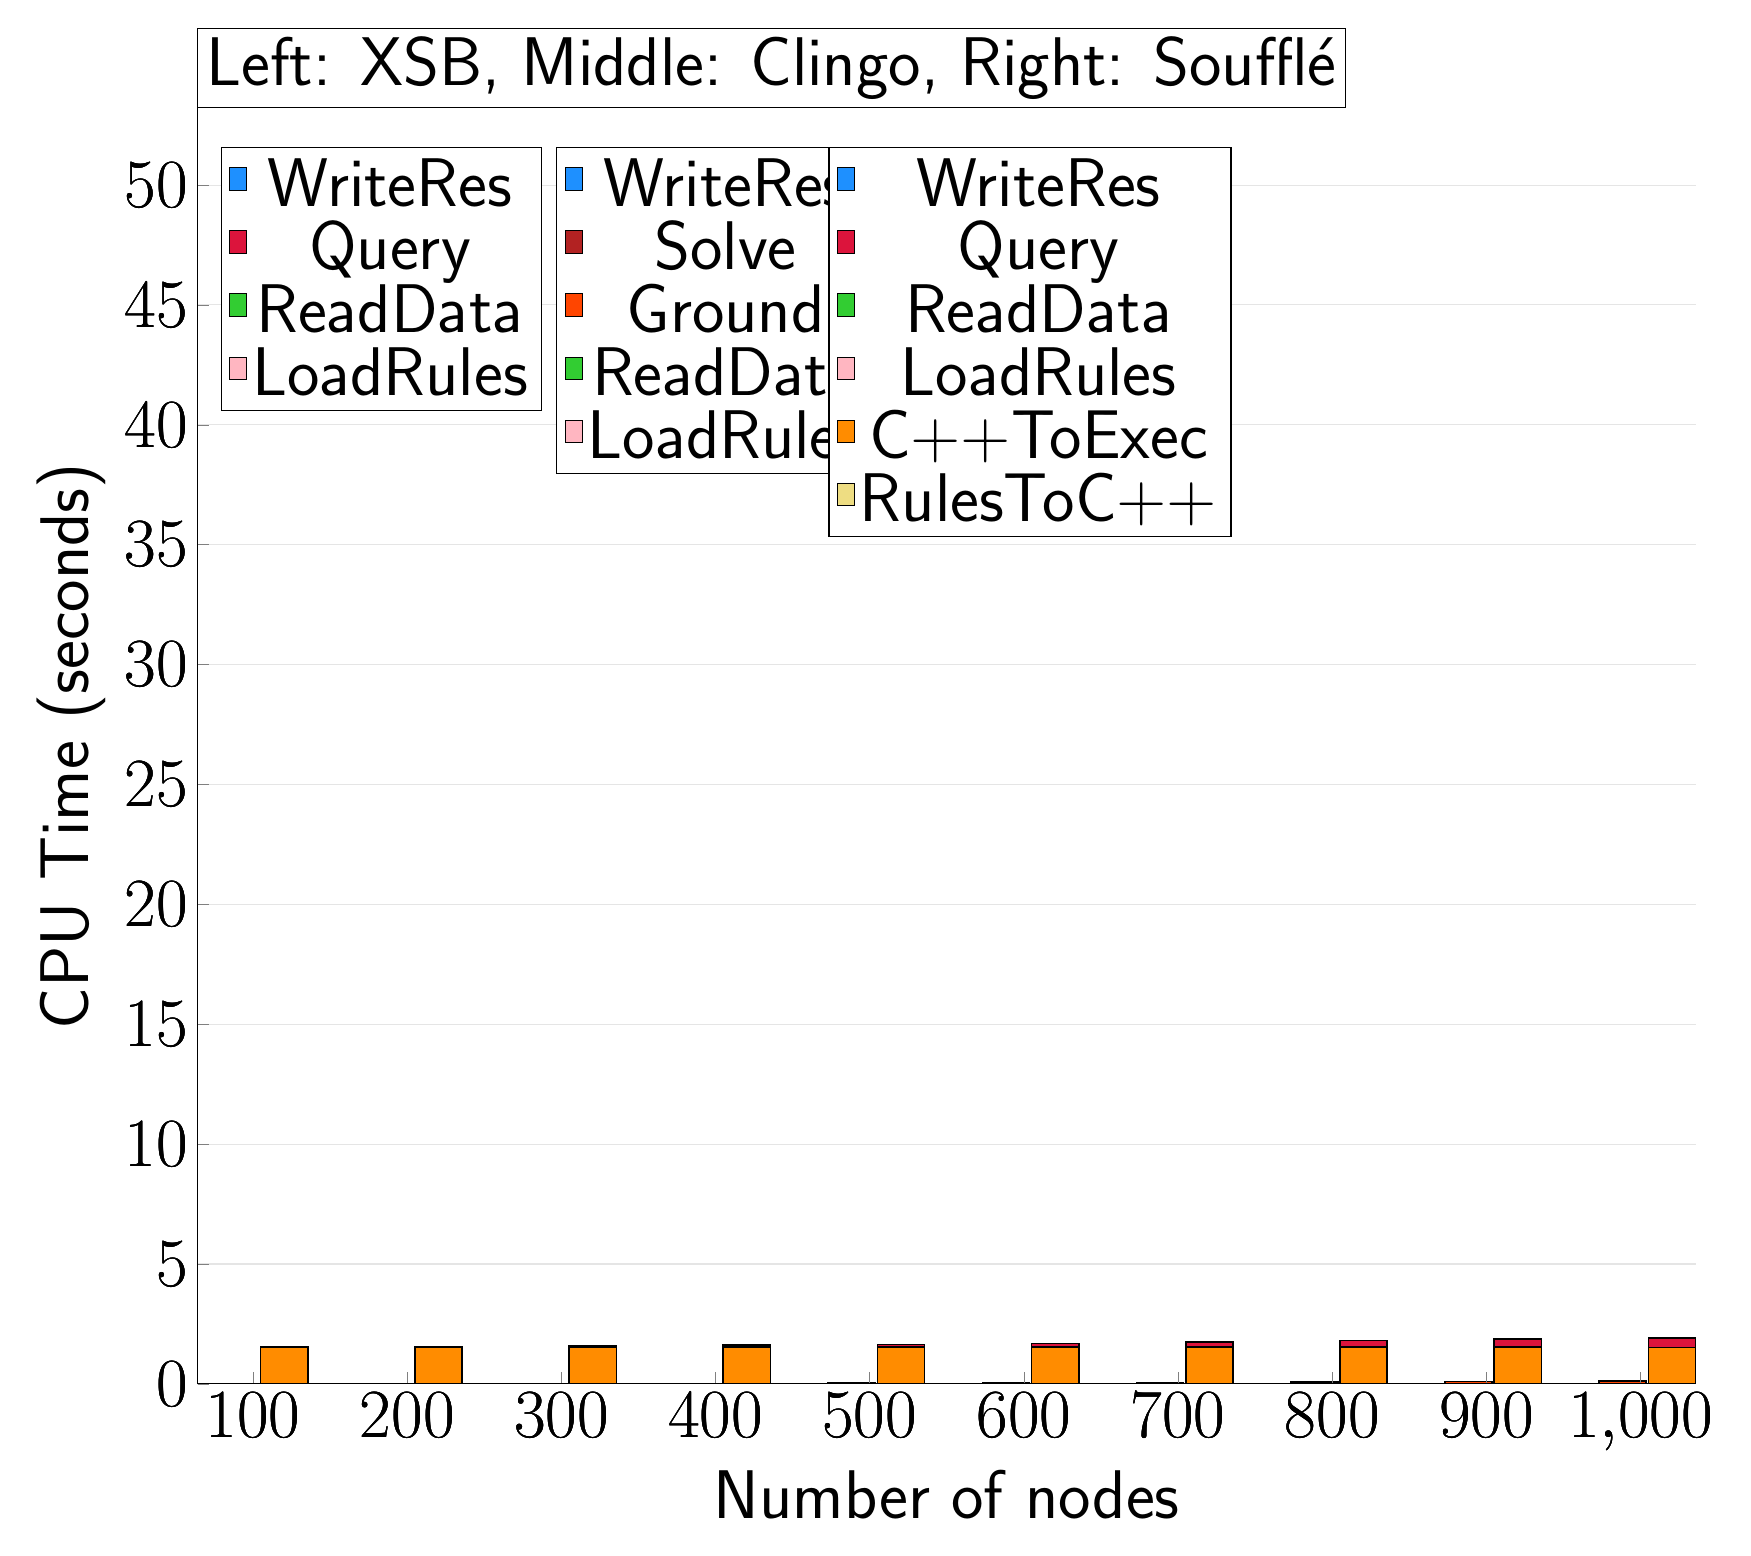
\begin{tikzpicture}
                        \begin{axis}[bar shift=-24.3pt, 
   ybar stacked,
   width=1.7\textwidth,
   bar width=0.6cm,
   ymajorgrids, tick align=inside,
   major grid style={draw=gray!20},
   xtick=data,
   ymin=0, ymax=53.1968,
   axis x line*=bottom,
   axis y line*=left,
   enlarge x limits=0.04,
   legend style={
       at={(0.23, 0.97)},
       anchor=north east,
       legend columns=1,
       font=\Huge,
   },
   ylabel={CPU Time (seconds)},
   xlabel={Number of nodes},
   label style={font=\Huge},
   tick label style={font=\Huge},
]
\addlegendimage{fill=DodgerBlue, draw=black, line width=0.2pt}
\addlegendentry{WriteRes}
\addlegendimage{fill=Crimson, draw=black, line width=0.2pt}
\addlegendentry{Query}
\addlegendimage{fill=LimeGreen, draw=black, line width=0.2pt}
\addlegendentry{ReadData}
\addlegendimage{fill=LightPink, draw=black, line width=0.2pt}
\addlegendentry{LoadRules}
\addplot +[fill=LightPink, draw=black, line width=0.55pt] coordinates {
(100, 0.0005555999999999998)
(200, 0.0005521999999999999)
(300, 0.0005499999999999994)
(400, 0.0005656000000000002)
(500, 0.0005526)
(600, 0.0005608000000000002)
(700, 0.0005542000000000005)
(800, 0.0005540000000000003)
(900, 0.0005580000000000003)
(1000, 0.0005531999999999995)
};
\addplot +[fill=LimeGreen, draw=black, line width=0.55pt] coordinates {
(100, 0.0002618)
(200, 0.00040800000000000065)
(300, 0.0005404000000000005)
(400, 0.0007084000000000002)
(500, 0.0008363999999999998)
(600, 0.0009814)
(700, 0.0011506000000000003)
(800, 0.0013055999999999999)
(900, 0.001487)
(1000, 0.001576)
};
\addplot +[fill=Crimson, draw=black, line width=0.55pt] coordinates {
(100, 2.0400000000000276e-05)
(200, 3.2199999999999604e-05)
(300, 4.240000000000008e-05)
(400, 6.199999999999991e-05)
(500, 7.239999999999988e-05)
(600, 8.679999999999972e-05)
(700, 9.75999999999994e-05)
(800, 0.00011300000000000019)
(900, 0.0001277999999999998)
(1000, 0.0001360000000000002)
};
\addplot +[fill=DodgerBlue, draw=black, line width=0.55pt] coordinates {
(100, 9.039999999999992e-05)
(200, 0.00011980000000000001)
(300, 0.00015180000000000033)
(400, 0.00018400000000000008)
(500, 0.0002106000000000001)
(600, 0.0002384000000000011)
(700, 0.0002746000000000002)
(800, 0.0003087999999999998)
(900, 0.0003396000000000008)
(1000, 0.00036120000000000016)
};
\end{axis}

\begin{axis}[bar shift=-6.5pt, 
   ybar stacked,
   width=1.7\textwidth,
   bar width=0.6cm,
   ymajorgrids, tick align=inside,
   major grid style={draw=none},
   xtick=data,
   ymin=0, ymax=53.1968,
   axis x line*=none,
   axis y line*=none,
   enlarge x limits=0.04,
   legend style={
       at={(0.454, 0.97)},
       anchor=north east,
       legend columns=1,
       font=\Huge,
   },
   label style={font=\Huge},
   tick label style={font=\Huge},
]
\addlegendimage{fill=DodgerBlue, draw=black, line width=0.2pt}
\addlegendentry{WriteRes}
\addlegendimage{fill=FireBrick, draw=black, line width=0.2pt}
\addlegendentry{Solve}
\addlegendimage{fill=OrangeRed, draw=black, line width=0.2pt}
\addlegendentry{Ground}
\addlegendimage{fill=LimeGreen, draw=black, line width=0.2pt}
\addlegendentry{ReadData}
\addlegendimage{fill=LightPink, draw=black, line width=0.2pt}
\addlegendentry{LoadRules}
\addplot +[fill=LightPink, draw=black, line width=0.55pt] coordinates {
(100, 0.0)
(200, 0.0)
(300, 0.0)
(400, 0.0)
(500, 0.0)
(600, 0.0)
(700, 0.0)
(800, 0.0)
(900, 0.0)
(1000, 0.0)
};
\addplot +[fill=LimeGreen, draw=black, line width=0.55pt] coordinates {
(100, 0.0)
(200, 0.0)
(300, 0.0)
(400, 0.0)
(500, 0.0)
(600, 0.0)
(700, 0.0040000000000000036)
(800, 0.0)
(900, 0.0)
(1000, 0.0)
};
\addplot +[fill=OrangeRed, draw=black, line width=0.55pt] coordinates {
(100, 0.0)
(200, 0.0040000000000000036)
(300, 0.010000000000000009)
(400, 0.020000000000000018)
(500, 0.030000000000000027)
(600, 0.040000000000000015)
(700, 0.055999999999999994)
(800, 0.07800000000000001)
(900, 0.10000000000000005)
(1000, 0.12)
};
\addplot +[fill=FireBrick, draw=black, line width=0.55pt] coordinates {
(100, 0.0)
(200, 0.0040000000000000036)
(300, 0.0)
(400, 0.0)
(500, 0.0)
(600, 0.0)
(700, 0.0020000000000000018)
(800, 0.0)
(900, 0.006000000000000005)
(1000, 0.0)
};
\addplot +[fill=DodgerBlue, draw=black, line width=0.55pt] coordinates {
(100, 0.0)
(200, -0.0040000000000000036)
(300, 0.0)
(400, 0.0)
(500, 0.0)
(600, 0.0)
(700, -1.3877787807814458e-18)
(800, 0.0020000000000000005)
(900, -0.0020000000000000018)
(1000, 0.0)
};
\end{axis}

\begin{axis}[bar shift=11.3pt, 
   ybar stacked,
   width=1.7\textwidth,
   bar width=0.6cm,
   ymajorgrids, tick align=inside,
   major grid style={draw=none},
   xtick=data,
   ymin=0, ymax=53.1968,
   axis x line*=none,
   axis y line*=none,
   enlarge x limits=0.04,
   legend style={
       at={(0.69, 0.97)},
       anchor=north east,
       legend columns=1,
       font=\Huge,
   },
   label style={font=\Huge},
   tick label style={font=\Huge},
]
\addlegendimage{fill=DodgerBlue, draw=black, line width=0.2pt}
\addlegendentry{WriteRes}
\addlegendimage{fill=Crimson, draw=black, line width=0.2pt}
\addlegendentry{Query}
\addlegendimage{fill=LimeGreen, draw=black, line width=0.2pt}
\addlegendentry{ReadData}
\addlegendimage{fill=LightPink, draw=black, line width=0.2pt}
\addlegendentry{LoadRules}
\addlegendimage{fill=DarkOrange, draw=black, line width=0.2pt}
\addlegendentry{C++ToExec}
\addlegendimage{fill=LightGoldenrod, draw=black, line width=0.2pt}
\addlegendentry{RulesToC++}
\addplot +[fill=LightGoldenrod, draw=black, line width=0.55pt] coordinates {
(100, 0.0)
(200, 0.0)
(300, 0.008000000000000002)
(400, 0.010000000000000002)
(500, 0.006000000000000001)
(600, 0.008000000000000002)
(700, 0.008000000000000002)
(800, 0.008000000000000002)
(900, 0.010000000000000002)
(1000, 0.007999999999999997)
};
\addplot +[fill=DarkOrange, draw=black, line width=0.55pt] coordinates {
(100, 1.5239999999999998)
(200, 1.518)
(300, 1.522)
(400, 1.518)
(500, 1.518)
(600, 1.52)
(700, 1.5259999999999998)
(800, 1.524)
(900, 1.518)
(1000, 1.5099999999999998)
};
\addplot +[fill=LightPink, draw=black, line width=0.55pt] coordinates {
(100, 0.00013919999999999997)
(200, 0.0001542)
(300, 0.00015079999999999998)
(400, 0.00014400000000000003)
(500, 0.0001514)
(600, 0.0001582)
(700, 0.00016659999999999998)
(800, 0.0001408)
(900, 0.000138)
(1000, 0.00013780000000000002)
};
\addplot +[fill=LimeGreen, draw=black, line width=0.55pt] coordinates {
(100, 0.0011224)
(200, 0.0019072)
(300, 0.0026236000000000002)
(400, 0.0030830000000000002)
(500, 0.003859)
(600, 0.0045462)
(700, 0.0055356)
(800, 0.005721200000000001)
(900, 0.005786399999999999)
(1000, 0.0060092)
};
\addplot +[fill=Crimson, draw=black, line width=0.55pt] coordinates {
(100, 0.0079308)
(200, 0.0260434)
(300, 0.049277)
(400, 0.079026)
(500, 0.1090152)
(600, 0.14812799999999998)
(700, 0.1991952)
(800, 0.261687)
(900, 0.3418558)
(1000, 0.388081)
};
\addplot +[fill=DodgerBlue, draw=black, line width=0.55pt] coordinates {
(100, 0.00027959999999999997)
(200, 0.0002854)
(300, 0.0002722)
(400, 0.00023960000000000002)
(500, 0.00028660000000000003)
(600, 0.0002804)
(700, 0.00030020000000000003)
(800, 0.0002954)
(900, 0.0003292)
(1000, 0.00035759999999999996)
};
\end{axis}


\node[anchor=south, draw, fill=white] at (rel axis cs:0.42,1) {\Huge Left: XSB, Middle: Clingo, Right: Soufflé};
\end{tikzpicture}
\end{document}
                    